\chapter{DBMS Functionalities and Architecture}
\section{Overview of a DBMS}
A database (DB) is a collection of homogeneous sets of data, with relationships defined among them, stored in a permanent memory and used by means of a  Data Base Management System (DBMS), a piece of software that provides the following key features:
\begin{itemize}
    \item A language for the database \textit{schema} definition. A collection of definitions which describe the data structure, the restrictions on allowable values of the data, and the relationships among data sets
    \item The data structures for the storage and efficient retrieval of large amounts of data in permanent memory
    \item The data structures for the storage and efficient retrieval of large amounts of data in permanent memory. Or to rapidly retrieve interesting subsets of the data from a specification of their features
    \item A transactions mechanism to protect data from hardware and software malfunctions and unwanted interference during concurrent access by multiple users
\end{itemize}

\newpage
\section{DBMS Architecture}
\begin{figure}[!h]
        \centering
        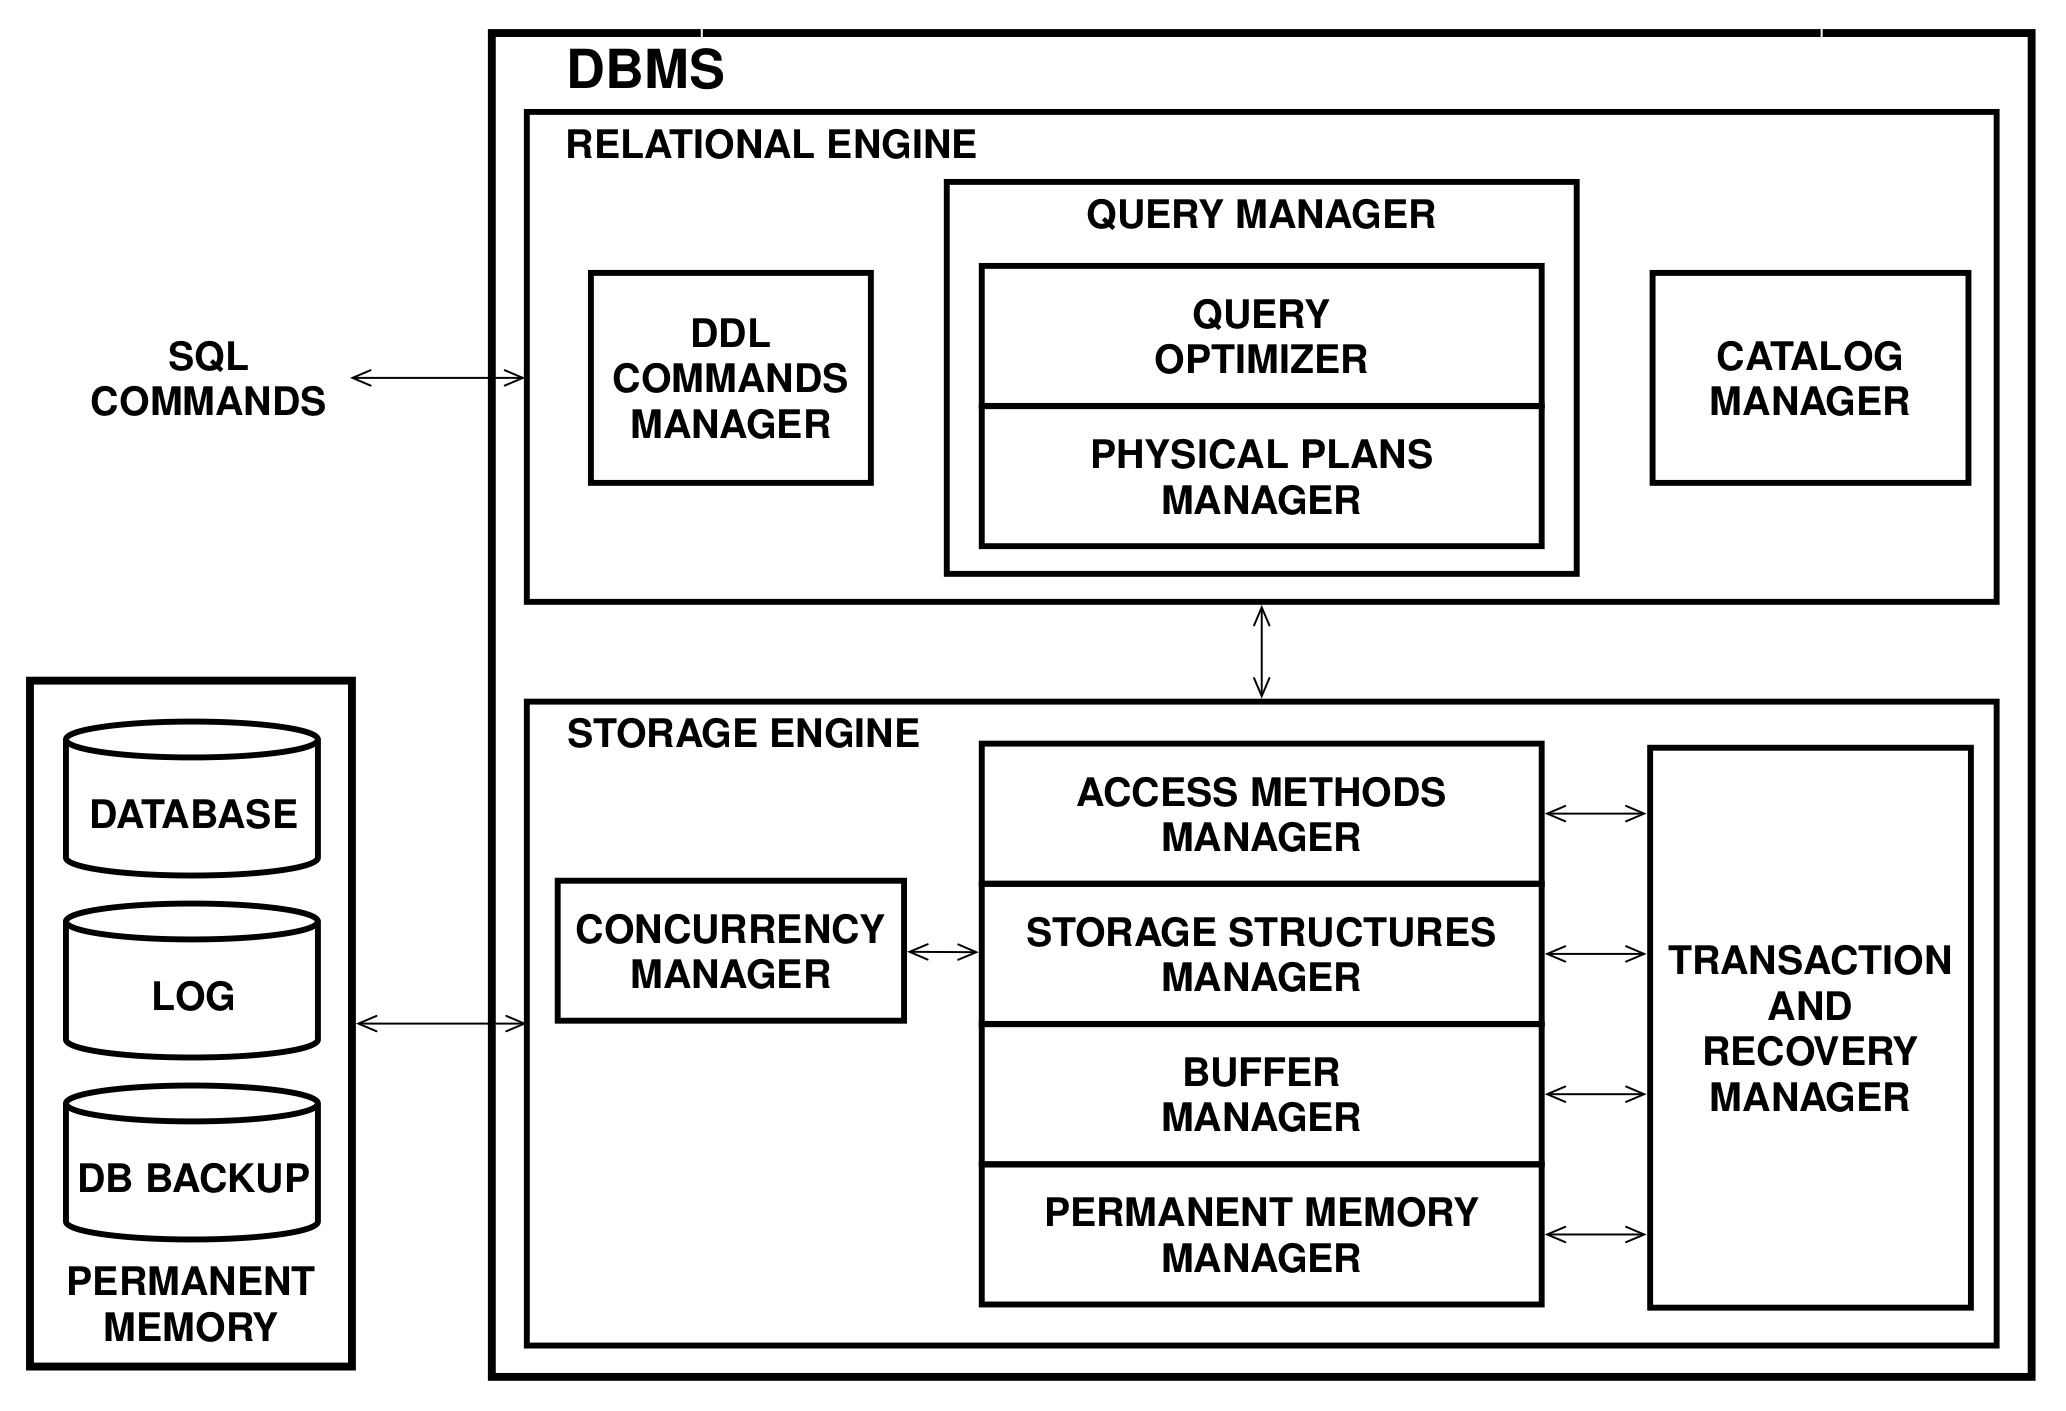
\includegraphics[width=0.7\linewidth]{images/DBMS_Internals/DBMS_architecture.jpeg}
        \caption{Architecture of a DBMS}
    \end{figure}

\begin{itemize}
    \item The \textbf{Storage Engine} which includes:
    \begin{itemize}
        \item The \textit{Permanent Memory Manager} which manages the page allocation and de-allocation on disk storage
        \item The \textit{Buffer Manager} which manages the transfer of data pages between the permanent memory and the main memory
        \item The \textit{Storage Structure Manager} which manages the data structures to store and retrieve data efficiently
        \item The \textit{Access Methods Manager} which provides the storage engine operators to create and destroy databases, files, indexes, and the data access methods for table scan, and index scan
        \item The \textit{Transaction and Recovery Manager} which ensures that the database’s consistency is maintained despite transaction and system failures
        \item The \textit{Concurrency Manager} which ensures that there is no conflict between concurrent access to the database.
    \end{itemize}
    \item The \textbf{Relational Engine} which includes:
    \begin{itemize}
        \item The \textit{Data Definition Language (DLL) Manager} which processes a user’s database schema definition 
        \item The \textit{Query Manager} which processes a user’s query by transforming it in to an equivalent but more efficient form
        \item The \textit{Catalog Manager} which manages special data, called metadata, about the schemas of the existing databases, and security and authorization
    \end{itemize}
\end{itemize}
Let us briefly examine the modules that will be considered in the following chapters:
\begin{itemize}
    \item The \textbf{Permanent Memory Manager} provides a vision of the memory as a set of databases each consisting of a set of files of physical pages of fixed size
    \item The \textbf{Buffer Manager} the execution cost of some queries can be reduced using a buffer capable of containing many pages, so that, while executing the queries, if there are repeated accesses to the same page, the likelihood that the desired page is already in memory increases
    \item The \textbf{Storage Structure Manager} provides the other system levels with a view of the permanent data organized into collections of records and indexes
    \item The \textbf{Access Methods Manager} provides a vision of permanent data organized in collections of records accessible one after the other in the order in which are stored, or through indexes, abstracting from their physical organization
    \item The \textbf{Transaction and Recovery Manager} provides the other system levels with a vision of the permanent memory as a set of pages in temporary memory without regard to failures 
    \item The \textbf{Concurrency Manager} provides the other system levels with a vision of permanent memory as a set pages in memory without regard to concurrent access, thus ensuring that the concurrent execution of several transactions takes place as if they were executed one after the other
    \item The \textbf{Query Manager} provides a vision of permanent data as a set of relational tables on which a user operates with SQL commands
\end{itemize}

\section{The JRS System}
The implementation of the relational DBMS modules will be discussed first in general and then with respect to the solutions adopted for the system JRS (Java Relational System), developed in Java at the Department of Computer Science, University of Pisa.

It is a simple system with all the most important components of a RDBMS, and its Java code can explored to learn about how such a system works.